\section{Digital to Analog Converter}
The final stage in the voice recording circuit is a digital to analog
converter, so that a standard audio speaker can be used to reproduce the
captured audio.
\subsection{Prediction}
\begin{figure}[H]
\centering
	\begin{tikzpicture}[gnuplot]
%% generated with GNUPLOT 4.4p2 (Lua 5.1.4; terminal rev. 97, script rev. 96a)
%% Tue 17 Jan 2012 05:45:50 PM EST
\gpsolidlines
\gpcolor{gp lt color border}
\gpsetlinetype{gp lt border}
\gpsetlinewidth{1.00}
\draw[gp path] (1.320,0.985)--(1.500,0.985);
\node[gp node right] at (1.136,0.985) {-16};
\draw[gp path] (1.320,1.461)--(1.500,1.461);
\node[gp node right] at (1.136,1.461) {-14};
\draw[gp path] (1.320,1.936)--(1.500,1.936);
\node[gp node right] at (1.136,1.936) {-12};
\draw[gp path] (1.320,2.412)--(1.500,2.412);
\node[gp node right] at (1.136,2.412) {-10};
\draw[gp path] (1.320,2.888)--(1.500,2.888);
\node[gp node right] at (1.136,2.888) {-8};
\draw[gp path] (1.320,3.363)--(1.500,3.363);
\node[gp node right] at (1.136,3.363) {-6};
\draw[gp path] (1.320,3.839)--(1.500,3.839);
\node[gp node right] at (1.136,3.839) {-4};
\draw[gp path] (1.320,4.314)--(1.500,4.314);
\node[gp node right] at (1.136,4.314) {-2};
\draw[gp path] (1.320,4.790)--(1.500,4.790);
\node[gp node right] at (1.136,4.790) { 0};
\draw[gp path] (1.320,0.985)--(1.320,1.165);
\node[gp node center] at (1.320,0.677) { 0};
\draw[gp path] (2.807,0.985)--(2.807,1.165);
\node[gp node center] at (2.807,0.677) { 5};
\draw[gp path] (4.294,0.985)--(4.294,1.165);
\node[gp node center] at (4.294,0.677) { 10};
\draw[gp path] (5.781,0.985)--(5.781,1.165);
\node[gp node center] at (5.781,0.677) { 15};
\draw[gp path] (7.268,0.985)--(7.268,1.165);
\node[gp node center] at (7.268,0.677) { 20};
\draw[gp path] (8.755,0.985)--(8.755,1.165);
\node[gp node center] at (8.755,0.677) { 25};
\draw[gp path] (10.242,0.985)--(10.242,1.165);
\node[gp node center] at (10.242,0.677) { 30};
\draw[gp path] (1.320,4.790)--(1.320,0.985)--(10.242,0.985);
\node[gp node center,rotate=-270] at (0.246,2.887) {Output Voltage, $V_\text{out}$ (\si{\volt})};
\node[gp node center] at (5.781,0.215) {Time, $t$ (\si{\micro\second})};
\node[gp node center] at (5.781,5.252) {DAC Output Prediction};
\gpcolor{gp lt color 0}
\gpsetlinetype{gp lt plot 0}
\draw[gp path] (1.320,4.790)--(1.410,4.790)--(1.500,4.790)--(1.590,4.790)--(1.680,4.790)%
  --(1.680,4.552)--(1.771,4.552)--(1.861,4.552)--(1.951,4.552)--(1.951,4.314)--(2.041,4.314)%
  --(2.131,4.314)--(2.221,4.314)--(2.221,4.077)--(2.311,4.077)--(2.401,4.077)--(2.492,4.077)%
  --(2.582,4.077)--(2.582,3.839)--(2.672,3.839)--(2.762,3.839)--(2.852,3.839)--(2.852,3.601)%
  --(2.942,3.601)--(3.032,3.601)--(3.122,3.601)--(3.122,3.363)--(3.213,3.363)--(3.303,3.363)%
  --(3.393,3.363)--(3.483,3.363)--(3.483,3.125)--(3.573,3.125)--(3.663,3.125)--(3.753,3.125)%
  --(3.753,2.888)--(3.843,2.888)--(3.934,2.888)--(4.024,2.888)--(4.024,2.650)--(4.114,2.650)%
  --(4.204,2.650)--(4.294,2.650)--(4.294,2.412)--(4.384,2.412)--(4.474,2.412)--(4.564,2.412)%
  --(4.654,2.412)--(4.654,2.174)--(4.745,2.174)--(4.835,2.174)--(4.925,2.174)--(4.925,1.936)%
  --(5.015,1.936)--(5.105,1.936)--(5.195,1.936)--(5.195,1.698)--(5.285,1.698)--(5.375,1.698)%
  --(5.466,1.698)--(5.556,1.698)--(5.556,1.461)--(5.646,1.461)--(5.736,1.461)--(5.826,1.461)%
  --(5.826,4.790)--(5.916,4.790)--(6.006,4.790)--(6.096,4.790)--(6.096,4.552)--(6.187,4.552)%
  --(6.277,4.552)--(6.367,4.552)--(6.457,4.552)--(6.457,4.314)--(6.547,4.314)--(6.637,4.314)%
  --(6.727,4.314)--(6.727,4.077)--(6.817,4.077)--(6.908,4.077)--(6.998,4.077)--(6.998,3.839)%
  --(7.088,3.839)--(7.178,3.839)--(7.268,3.839)--(7.268,3.601)--(7.358,3.601)--(7.448,3.601)%
  --(7.538,3.601)--(7.628,3.601)--(7.628,3.363)--(7.719,3.363)--(7.809,3.363)--(7.899,3.363)%
  --(7.899,3.125)--(7.989,3.125)--(8.079,3.125)--(8.169,3.125)--(8.169,2.888)--(8.259,2.888)%
  --(8.349,2.888)--(8.440,2.888)--(8.530,2.888)--(8.530,2.650)--(8.620,2.650)--(8.710,2.650)%
  --(8.800,2.650)--(8.800,2.412)--(8.890,2.412)--(8.980,2.412)--(9.070,2.412)--(9.070,2.174)%
  --(9.161,2.174)--(9.251,2.174)--(9.341,2.174)--(9.431,2.174)--(9.431,1.936)--(9.521,1.936)%
  --(9.611,1.936)--(9.701,1.936)--(9.701,1.698)--(9.791,1.698)--(9.882,1.698)--(9.972,1.698)%
  --(9.972,1.461)--(10.062,1.461)--(10.152,1.461)--(10.242,1.461)--(10.242,4.790);
\gpcolor{gp lt color border}
\gpsetlinetype{gp lt border}
\draw[gp path] (1.320,4.790)--(1.320,0.985)--(10.242,0.985);
%% coordinates of the plot area
\gpdefrectangularnode{gp plot 1}{\pgfpoint{1.320cm}{0.985cm}}{\pgfpoint{10.242cm}{4.790cm}}
\end{tikzpicture}
%% gnuplot variables

\end{figure}
% TODO: Prediction graph

\subsection{Discrete DAC Simulation}
The provided DAC schematic was captured in Cadence PSpice as shown in
Figure~\ref{f:dac_schem}.
%
\begin{figure}[H]
\centering
	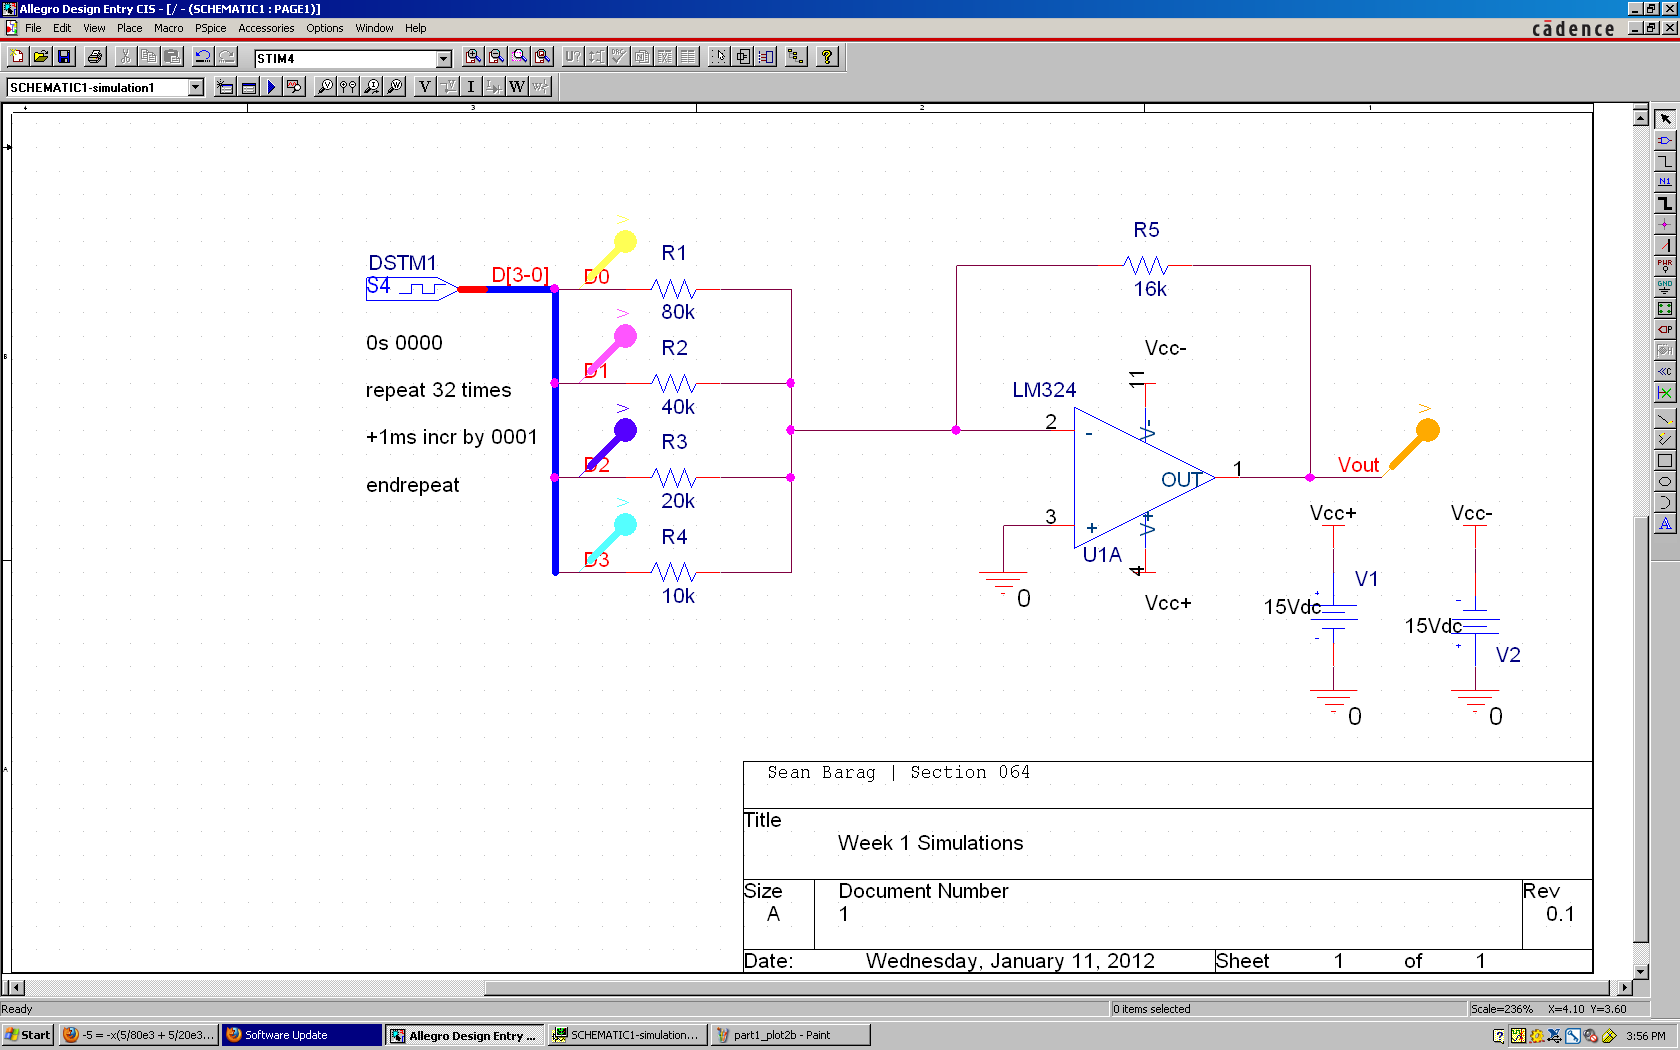
\includegraphics[width=.8\textwidth]{img/shot/part1_schem.PNG}
	\parbox{.8\textwidth}{
	\caption[Discrete DAC --- Schematic]{Provided schematic for the discrete
	digital to analog converter (DAC).  Note that the value of~$R_5$ has
	already been adjusted in this image.}
	\label{f:dac_schem}}
\end{figure}
%
Note that the element titled ``DTSM 1'' was edited to repeatedly count from
zero~($0000_2$) to fifteen~($1111_2$) with each intermediate value
lasting for~\SI{1}{\milli\second}.  This was accomplished by editing the
element properties and providing the four instructions shown:
%
\begin{itemize*}
	\item \ttt{0s 0000}
	\item \ttt{repeat 32 times}
	\item \ttt{+1ms incr by 00001}
	\item \ttt{endrepeat}
\end{itemize*}
%
This circuit was simulated using transient analysis for the
required~\SI{32}{\milli\second}, allowing one full input count-up cycle to be
observed.  The voltage at each bit, along with the output voltage, is plotted
below in Figure~\ref{f:dac_plot1}.
%
\begin{figure}[H]
\centering
	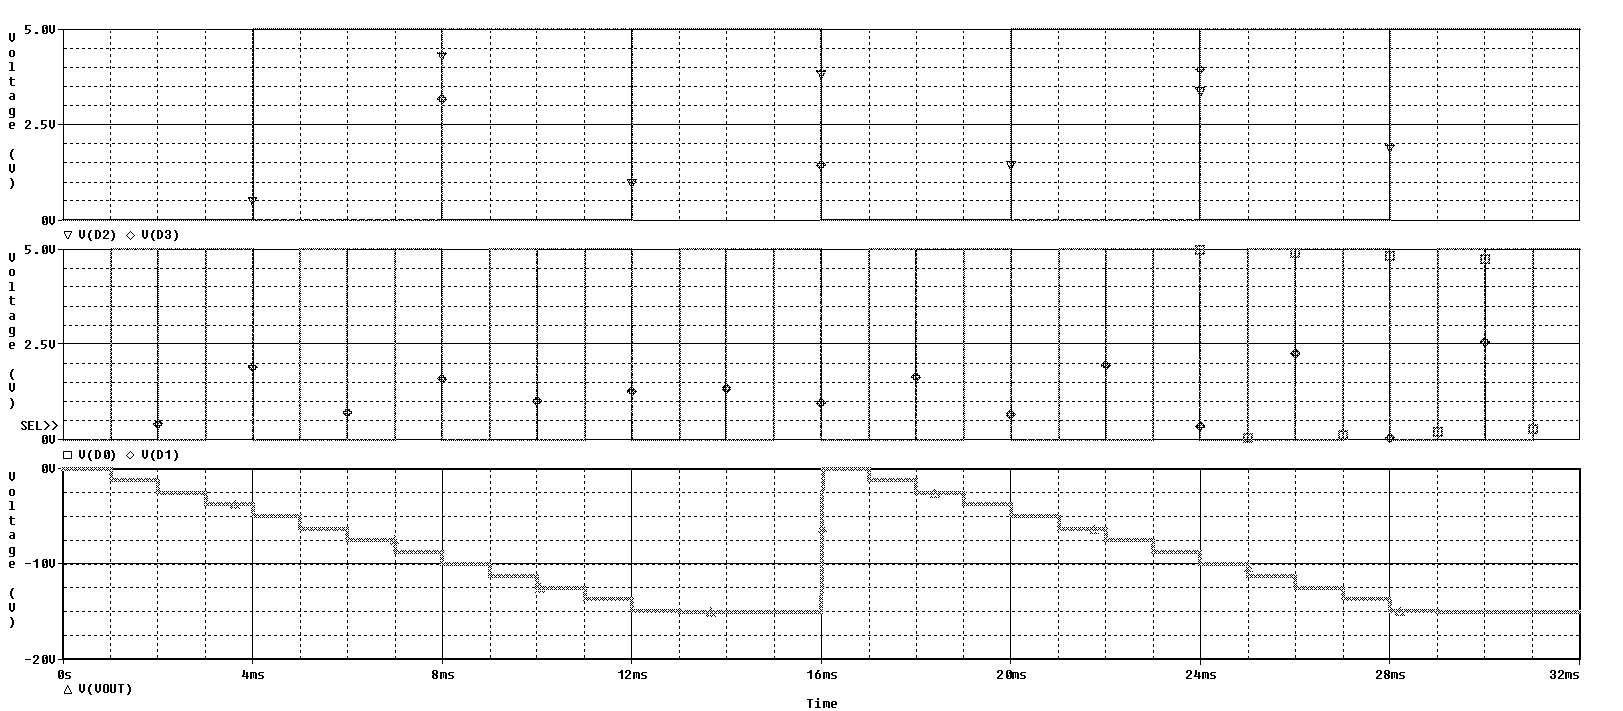
\includegraphics[width=.8\textwidth]{img/plot/part1_plot1b.PNG}
	\parbox{.8\textwidth}{
	\caption[Discrete DAC --- Initial Results]{Initial simulation results for
	the discrete DAC.  Note that the output reaches a lower threshold as a
	result of the value of~$R_5$.}
	\label{f:dac_plot1}}
\end{figure}
%
As is shown in the produced plot of output voltage versus time, the output
reaches the minimum possible output voltage of~\SI{-15}{\volt}
at~\SI{12}{\milli\second}.  This is caused by an improperly tuned feedback
resistor~$R_5$.

\subsection{Feedback Resistor Tuning}
In order to ensure that the minimum output voltage of~\SI{-15}{\volt}~(limited
by the op amp's supply voltage) occurs at the maximum input value of~$1111_2$,
the value of the feedback resistor~$R_5$ must be adjusted.  The output voltage
of the discrete DAC is governed by~\eqref{eq:dac}:
%
\begin{equation}
	V_\text{out} = - 5 R_5 \left( \frac{D_3}{R_4} + \frac{D_2}{R_3} + \frac{D_1}{R_2} + \frac{D_0}{R_1} \right)
	\label{eq:dac}
\end{equation}
%
where~$D_0$ through~$D_3$ are the binary values of the corresponding bits in
Figure~\ref{f:dac_schem} and~$R_1$ through~$R_5$ are the associated resistors
in the same schematic.  Note that the negative sign on the right-hand side is a
result of using the inverting terminal of the opamp for our varying input.  By
designing for a binary value of~0101 to correspond with a~\SI{-5}{\volt}
output, we can ensure that the full-scale output will fall at~\SI{-15}{\volt}.
%
\begin{align*}
	V_\text{out} = \SI{-5}{\volt} &= -5 R_5 \left( \frac{0}{\SI{10}{\kilo\ohm}} + \frac{1}{\SI{20}{\kilo\ohm}} + \frac{0}{\SI{40}{\kilo\ohm}} + \frac{1}{\SI{80}{\kilo\ohm}} \right) \\
	R_5 &= \frac{ -5 } { -5 \left( \frac{1}{\SI{20}{\kilo\ohm}} + \frac{1}{\SI{80}{\kilo\ohm}} \right) } \\
	    &= \SI{16}{\kilo\ohm}
\end{align*}
%
After completing these calculations, an appropriate value of~$R_5$ was
determined to be~\SI{16}{\volt}.

\subsection{Adjusted DAC Simulation}
The value of~$R_5$ was changed in the schematic and the simulation was run
again with the same~\SI{32}{\milli\second} duration.  Upon the simulation's
completion, PSpice produced the plot shown in Figure~\ref{f:dac_plot2}, below.
%
\begin{figure}[H]
\centering
	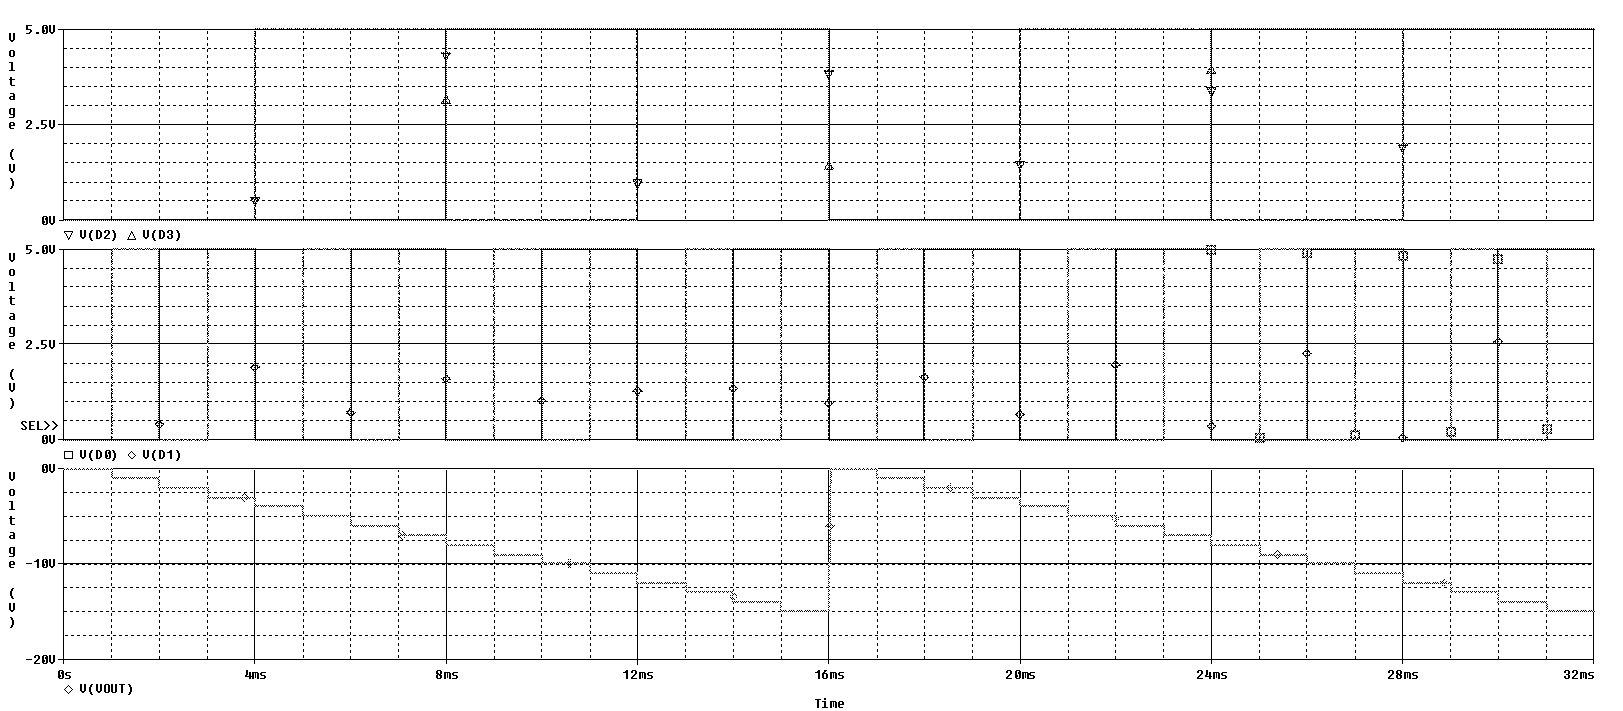
\includegraphics[width=.8\textwidth]{img/plot/part1_plot2b.PNG}
	\parbox{.8\textwidth}{
	\caption[Discrete DAC --- Tuned Results]{Final simulation results with an
	adjusted feedback resistor.}
	\label{f:dac_plot2}}
\end{figure}

\subsection{Discrete DAC Results}
As is shown in the above included PSpice plot, the digital to analog converter
produces an accurate representation of the input bits.  By adjusting the value
of the feedback resistor, students were able to ensure that the full-scale
input produced an output voltage within the range of values that could be
accurately represented.  The supply voltages for the operational amplifier
determined the maximum and minimum possible outputs, thus requiring students to
force a full-scale input of~$0000_2$ to~\SI{-15}{\volt} or more.  The output
waveform shows that for each increase in input value there is a corresponding
decrease in output voltage, a voltage difference that remains constant through
the entire range of inputs at roughly~\SI{-1}{\volt\per\bit}.
